% Created by tikzDevice version 0.7.0 on 2014-07-24 03:38:07
% !TEX encoding = UTF-8 Unicode
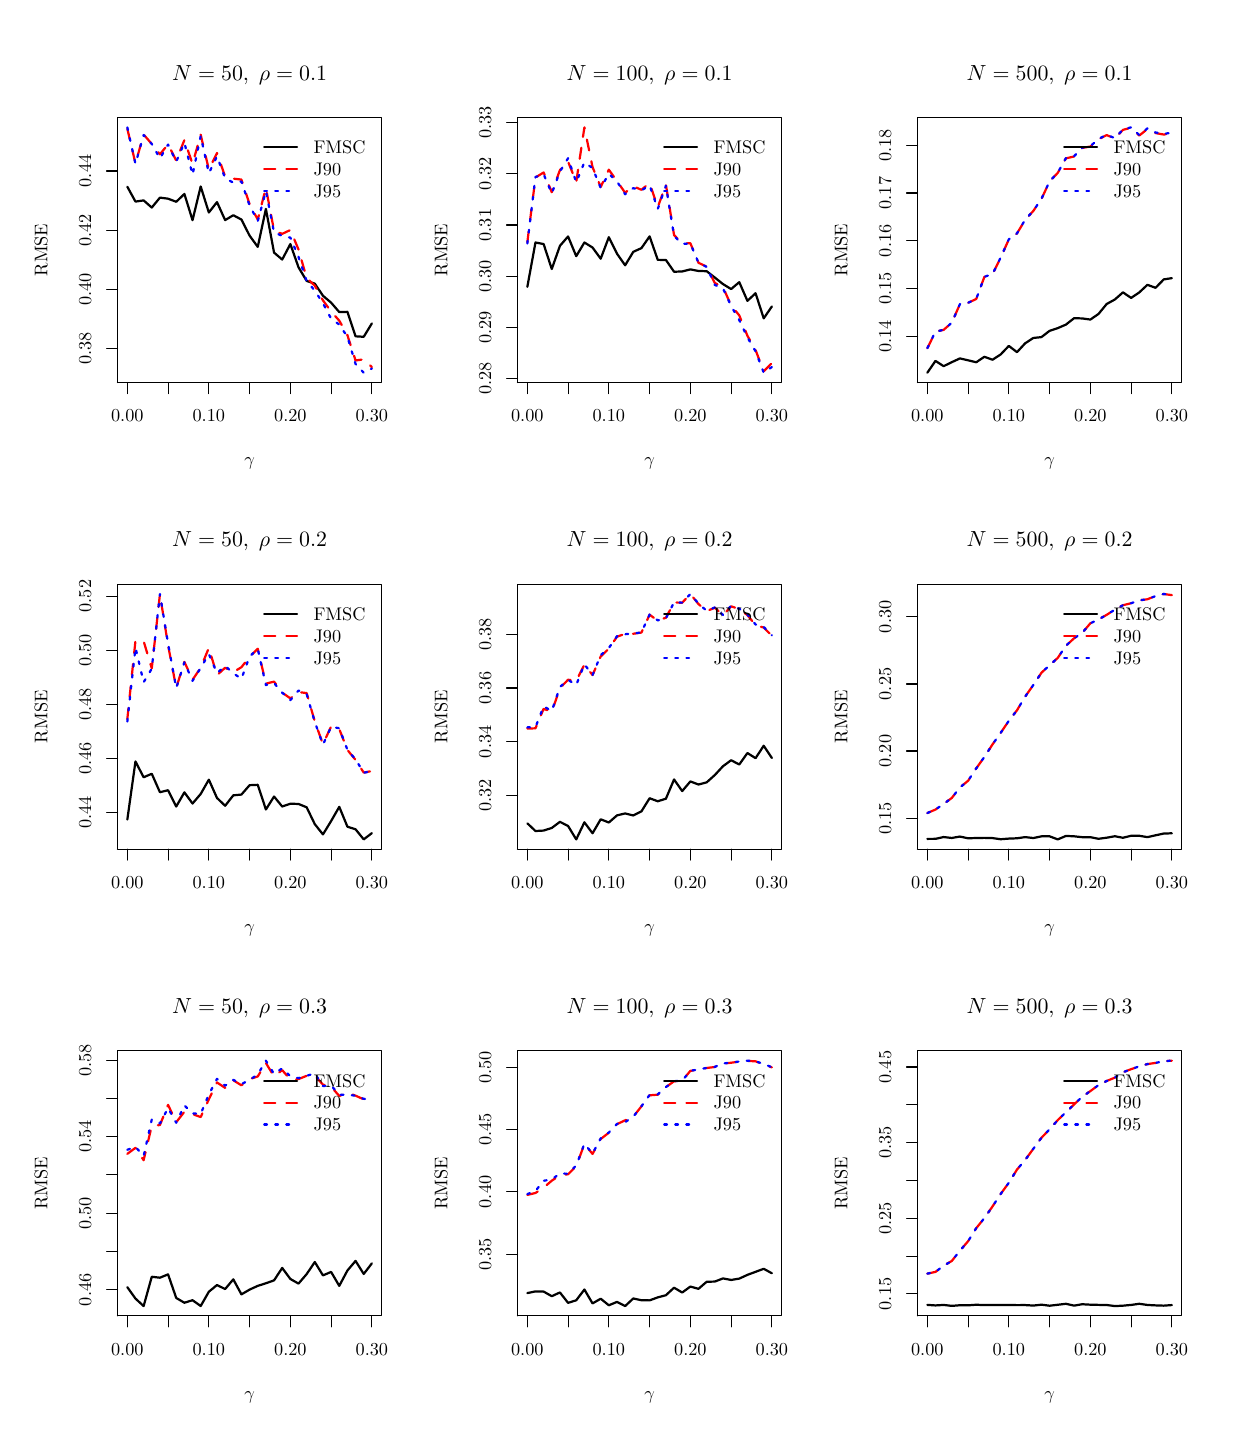
\begin{tikzpicture}[x=1pt,y=1pt]
\definecolor[named]{fillColor}{rgb}{1.00,1.00,1.00}
\path[use as bounding box,fill=fillColor,fill opacity=0.00] (0,0) rectangle (433.62,505.89);
\begin{scope}
\path[clip] ( 32.47,377.65) rectangle (127.91,473.42);
\definecolor[named]{drawColor}{rgb}{0.00,0.00,0.00}

\path[draw=drawColor,line width= 0.8pt,line join=round,line cap=round] ( 36.01,448.40) --
	( 38.95,443.04) --
	( 41.90,443.47) --
	( 44.84,440.88) --
	( 47.79,444.47) --
	( 50.73,444.09) --
	( 53.68,442.97) --
	( 56.63,445.80) --
	( 59.57,436.32) --
	( 62.52,448.50) --
	( 65.46,439.10) --
	( 68.41,442.85) --
	( 71.35,436.35) --
	( 74.30,438.11) --
	( 77.24,436.55) --
	( 80.19,430.73) --
	( 83.14,426.68) --
	( 86.08,440.41) --
	( 89.03,424.60) --
	( 91.97,422.10) --
	( 94.92,427.70) --
	( 97.86,419.31) --
	(100.81,414.37) --
	(103.75,413.40) --
	(106.70,409.01) --
	(109.65,406.52) --
	(112.59,403.11) --
	(115.54,403.20) --
	(118.48,394.36) --
	(121.43,394.18) --
	(124.37,399.02);
\end{scope}
\begin{scope}
\path[clip] (  0.00,  0.00) rectangle (433.62,505.89);
\definecolor[named]{drawColor}{rgb}{0.00,0.00,0.00}

\path[draw=drawColor,line width= 0.4pt,line join=round,line cap=round] ( 36.01,377.65) -- (124.37,377.65);

\path[draw=drawColor,line width= 0.4pt,line join=round,line cap=round] ( 36.01,377.65) -- ( 36.01,373.69);

\path[draw=drawColor,line width= 0.4pt,line join=round,line cap=round] ( 50.73,377.65) -- ( 50.73,373.69);

\path[draw=drawColor,line width= 0.4pt,line join=round,line cap=round] ( 65.46,377.65) -- ( 65.46,373.69);

\path[draw=drawColor,line width= 0.4pt,line join=round,line cap=round] ( 80.19,377.65) -- ( 80.19,373.69);

\path[draw=drawColor,line width= 0.4pt,line join=round,line cap=round] ( 94.92,377.65) -- ( 94.92,373.69);

\path[draw=drawColor,line width= 0.4pt,line join=round,line cap=round] (109.65,377.65) -- (109.65,373.69);

\path[draw=drawColor,line width= 0.4pt,line join=round,line cap=round] (124.37,377.65) -- (124.37,373.69);

\node[text=drawColor,anchor=base,inner sep=0pt, outer sep=0pt, scale=  0.66] at ( 36.01,363.40) {0.00};

\node[text=drawColor,anchor=base,inner sep=0pt, outer sep=0pt, scale=  0.66] at ( 65.46,363.40) {0.10};

\node[text=drawColor,anchor=base,inner sep=0pt, outer sep=0pt, scale=  0.66] at ( 94.92,363.40) {0.20};

\node[text=drawColor,anchor=base,inner sep=0pt, outer sep=0pt, scale=  0.66] at (124.37,363.40) {0.30};

\path[draw=drawColor,line width= 0.4pt,line join=round,line cap=round] ( 32.47,389.93) -- ( 32.47,454.11);

\path[draw=drawColor,line width= 0.4pt,line join=round,line cap=round] ( 32.47,389.93) -- ( 28.51,389.93);

\path[draw=drawColor,line width= 0.4pt,line join=round,line cap=round] ( 32.47,411.32) -- ( 28.51,411.32);

\path[draw=drawColor,line width= 0.4pt,line join=round,line cap=round] ( 32.47,432.72) -- ( 28.51,432.72);

\path[draw=drawColor,line width= 0.4pt,line join=round,line cap=round] ( 32.47,454.11) -- ( 28.51,454.11);

\node[text=drawColor,rotate= 90.00,anchor=base,inner sep=0pt, outer sep=0pt, scale=  0.66] at ( 22.97,389.93) {0.38};

\node[text=drawColor,rotate= 90.00,anchor=base,inner sep=0pt, outer sep=0pt, scale=  0.66] at ( 22.97,411.32) {0.40};

\node[text=drawColor,rotate= 90.00,anchor=base,inner sep=0pt, outer sep=0pt, scale=  0.66] at ( 22.97,432.72) {0.42};

\node[text=drawColor,rotate= 90.00,anchor=base,inner sep=0pt, outer sep=0pt, scale=  0.66] at ( 22.97,454.11) {0.44};

\path[draw=drawColor,line width= 0.4pt,line join=round,line cap=round] ( 32.47,377.65) --
	(127.91,377.65) --
	(127.91,473.42) --
	( 32.47,473.42) --
	( 32.47,377.65);
\end{scope}
\begin{scope}
\path[clip] (  0.00,337.26) rectangle (144.54,505.89);
\definecolor[named]{drawColor}{rgb}{0.00,0.00,0.00}

\node[text=drawColor,anchor=base,inner sep=0pt, outer sep=0pt, scale=  0.79] at ( 80.19,486.92) {\bfseries $N=50, \;\rho=0.1$};

\node[text=drawColor,anchor=base,inner sep=0pt, outer sep=0pt, scale=  0.66] at ( 80.19,347.56) {$\gamma$};

\node[text=drawColor,rotate= 90.00,anchor=base,inner sep=0pt, outer sep=0pt, scale=  0.66] at (  7.13,425.53) {RMSE};
\end{scope}
\begin{scope}
\path[clip] ( 32.47,377.65) rectangle (127.91,473.42);
\definecolor[named]{drawColor}{rgb}{1.00,0.00,0.00}

\path[draw=drawColor,line width= 0.8pt,dash pattern=on 4pt off 4pt ,line join=round,line cap=round] ( 36.01,469.35) --
	( 38.95,456.83) --
	( 41.90,467.26) --
	( 44.84,463.89) --
	( 47.79,460.13) --
	( 50.73,463.73) --
	( 53.68,457.89) --
	( 56.63,465.27) --
	( 59.57,456.67) --
	( 62.52,467.21) --
	( 65.46,454.64) --
	( 68.41,460.59) --
	( 71.35,452.09) --
	( 74.30,451.33) --
	( 77.24,450.99) --
	( 80.19,442.11) --
	( 83.14,436.54) --
	( 86.08,447.99) --
	( 89.03,432.52) --
	( 91.97,431.38) --
	( 94.92,432.77) --
	( 97.86,425.75) --
	(100.81,415.41) --
	(103.75,412.67) --
	(106.70,407.35) --
	(109.65,403.30) --
	(112.59,400.03) --
	(115.54,394.76) --
	(118.48,385.62) --
	(121.43,386.05) --
	(124.37,383.24);
\definecolor[named]{drawColor}{rgb}{0.00,0.00,1.00}

\path[draw=drawColor,line width= 0.8pt,dash pattern=on 1pt off 3pt ,line join=round,line cap=round] ( 36.01,469.87) --
	( 38.95,456.69) --
	( 41.90,467.11) --
	( 44.84,463.88) --
	( 47.79,458.63) --
	( 50.73,463.64) --
	( 53.68,457.45) --
	( 56.63,464.32) --
	( 59.57,452.73) --
	( 62.52,466.71) --
	( 65.46,453.28) --
	( 68.41,459.37) --
	( 71.35,451.48) --
	( 74.30,449.88) --
	( 77.24,450.29) --
	( 80.19,441.60) --
	( 83.14,435.99) --
	( 86.08,446.82) --
	( 89.03,431.92) --
	( 91.97,430.65) --
	( 94.92,430.02) --
	( 97.86,423.10) --
	(100.81,414.32) --
	(103.75,410.89) --
	(106.70,406.27) --
	(109.65,400.76) --
	(112.59,398.60) --
	(115.54,394.17) --
	(118.48,384.36) --
	(121.43,381.20) --
	(124.37,382.71);
\definecolor[named]{drawColor}{rgb}{0.00,0.00,0.00}

\path[draw=drawColor,line width= 0.8pt,line join=round,line cap=round] ( 85.47,462.63) -- ( 97.35,462.63);
\definecolor[named]{drawColor}{rgb}{1.00,0.00,0.00}

\path[draw=drawColor,line width= 0.8pt,dash pattern=on 4pt off 4pt ,line join=round,line cap=round] ( 85.47,454.71) -- ( 97.35,454.71);
\definecolor[named]{drawColor}{rgb}{0.00,0.00,1.00}

\path[draw=drawColor,line width= 0.8pt,dash pattern=on 1pt off 3pt ,line join=round,line cap=round] ( 85.47,446.79) -- ( 97.35,446.79);
\definecolor[named]{drawColor}{rgb}{0.00,0.00,0.00}

\node[text=drawColor,anchor=base west,inner sep=0pt, outer sep=0pt, scale=  0.66] at (103.29,460.35) {FMSC};

\node[text=drawColor,anchor=base west,inner sep=0pt, outer sep=0pt, scale=  0.66] at (103.29,452.43) {J90};

\node[text=drawColor,anchor=base west,inner sep=0pt, outer sep=0pt, scale=  0.66] at (103.29,444.51) {J95};
\end{scope}
\begin{scope}
\path[clip] (177.01,377.65) rectangle (272.45,473.42);
\definecolor[named]{drawColor}{rgb}{0.00,0.00,0.00}

\path[draw=drawColor,line width= 0.8pt,line join=round,line cap=round] (180.55,412.23) --
	(183.49,428.26) --
	(186.44,427.69) --
	(189.38,418.68) --
	(192.33,427.06) --
	(195.27,430.44) --
	(198.22,423.31) --
	(201.17,428.26) --
	(204.11,426.44) --
	(207.06,422.40) --
	(210.00,430.17) --
	(212.95,424.21) --
	(215.89,420.02) --
	(218.84,424.89) --
	(221.78,426.22) --
	(224.73,430.47) --
	(227.68,421.98) --
	(230.62,421.95) --
	(233.57,417.69) --
	(236.51,417.79) --
	(239.46,418.54) --
	(242.40,417.97) --
	(245.35,417.88) --
	(248.29,415.59) --
	(251.24,413.24) --
	(254.19,411.43) --
	(257.13,413.93) --
	(260.08,407.17) --
	(263.02,409.93) --
	(265.97,400.84) --
	(268.91,405.14);
\end{scope}
\begin{scope}
\path[clip] (  0.00,  0.00) rectangle (433.62,505.89);
\definecolor[named]{drawColor}{rgb}{0.00,0.00,0.00}

\path[draw=drawColor,line width= 0.4pt,line join=round,line cap=round] (180.55,377.65) -- (268.91,377.65);

\path[draw=drawColor,line width= 0.4pt,line join=round,line cap=round] (180.55,377.65) -- (180.55,373.69);

\path[draw=drawColor,line width= 0.4pt,line join=round,line cap=round] (195.27,377.65) -- (195.27,373.69);

\path[draw=drawColor,line width= 0.4pt,line join=round,line cap=round] (210.00,377.65) -- (210.00,373.69);

\path[draw=drawColor,line width= 0.4pt,line join=round,line cap=round] (224.73,377.65) -- (224.73,373.69);

\path[draw=drawColor,line width= 0.4pt,line join=round,line cap=round] (239.46,377.65) -- (239.46,373.69);

\path[draw=drawColor,line width= 0.4pt,line join=round,line cap=round] (254.19,377.65) -- (254.19,373.69);

\path[draw=drawColor,line width= 0.4pt,line join=round,line cap=round] (268.91,377.65) -- (268.91,373.69);

\node[text=drawColor,anchor=base,inner sep=0pt, outer sep=0pt, scale=  0.66] at (180.55,363.40) {0.00};

\node[text=drawColor,anchor=base,inner sep=0pt, outer sep=0pt, scale=  0.66] at (210.00,363.40) {0.10};

\node[text=drawColor,anchor=base,inner sep=0pt, outer sep=0pt, scale=  0.66] at (239.46,363.40) {0.20};

\node[text=drawColor,anchor=base,inner sep=0pt, outer sep=0pt, scale=  0.66] at (268.91,363.40) {0.30};

\path[draw=drawColor,line width= 0.4pt,line join=round,line cap=round] (177.01,379.18) -- (177.01,471.53);

\path[draw=drawColor,line width= 0.4pt,line join=round,line cap=round] (177.01,379.18) -- (173.05,379.18);

\path[draw=drawColor,line width= 0.4pt,line join=round,line cap=round] (177.01,397.65) -- (173.05,397.65);

\path[draw=drawColor,line width= 0.4pt,line join=round,line cap=round] (177.01,416.12) -- (173.05,416.12);

\path[draw=drawColor,line width= 0.4pt,line join=round,line cap=round] (177.01,434.59) -- (173.05,434.59);

\path[draw=drawColor,line width= 0.4pt,line join=round,line cap=round] (177.01,453.06) -- (173.05,453.06);

\path[draw=drawColor,line width= 0.4pt,line join=round,line cap=round] (177.01,471.53) -- (173.05,471.53);

\node[text=drawColor,rotate= 90.00,anchor=base,inner sep=0pt, outer sep=0pt, scale=  0.66] at (167.51,379.18) {0.28};

\node[text=drawColor,rotate= 90.00,anchor=base,inner sep=0pt, outer sep=0pt, scale=  0.66] at (167.51,397.65) {0.29};

\node[text=drawColor,rotate= 90.00,anchor=base,inner sep=0pt, outer sep=0pt, scale=  0.66] at (167.51,416.12) {0.30};

\node[text=drawColor,rotate= 90.00,anchor=base,inner sep=0pt, outer sep=0pt, scale=  0.66] at (167.51,434.59) {0.31};

\node[text=drawColor,rotate= 90.00,anchor=base,inner sep=0pt, outer sep=0pt, scale=  0.66] at (167.51,453.06) {0.32};

\node[text=drawColor,rotate= 90.00,anchor=base,inner sep=0pt, outer sep=0pt, scale=  0.66] at (167.51,471.53) {0.33};

\path[draw=drawColor,line width= 0.4pt,line join=round,line cap=round] (177.01,377.65) --
	(272.45,377.65) --
	(272.45,473.42) --
	(177.01,473.42) --
	(177.01,377.65);
\end{scope}
\begin{scope}
\path[clip] (144.54,337.26) rectangle (289.08,505.89);
\definecolor[named]{drawColor}{rgb}{0.00,0.00,0.00}

\node[text=drawColor,anchor=base,inner sep=0pt, outer sep=0pt, scale=  0.79] at (224.73,486.92) {\bfseries $N=100, \;\rho=0.1$};

\node[text=drawColor,anchor=base,inner sep=0pt, outer sep=0pt, scale=  0.66] at (224.73,347.56) {$\gamma$};

\node[text=drawColor,rotate= 90.00,anchor=base,inner sep=0pt, outer sep=0pt, scale=  0.66] at (151.67,425.54) {RMSE};
\end{scope}
\begin{scope}
\path[clip] (177.01,377.65) rectangle (272.45,473.42);
\definecolor[named]{drawColor}{rgb}{1.00,0.00,0.00}

\path[draw=drawColor,line width= 0.8pt,dash pattern=on 4pt off 4pt ,line join=round,line cap=round] (180.55,428.35) --
	(183.49,451.74) --
	(186.44,453.56) --
	(189.38,446.43) --
	(192.33,454.42) --
	(195.27,457.48) --
	(198.22,450.08) --
	(201.17,469.87) --
	(204.11,455.52) --
	(207.06,448.32) --
	(210.00,454.57) --
	(212.95,450.43) --
	(215.89,446.24) --
	(218.84,448.57) --
	(221.78,447.30) --
	(224.73,449.76) --
	(227.68,441.01) --
	(230.62,449.17) --
	(233.57,430.96) --
	(236.51,427.87) --
	(239.46,427.99) --
	(242.40,420.92) --
	(245.35,419.53) --
	(248.29,413.62) --
	(251.24,412.15) --
	(254.19,405.51) --
	(257.13,401.92) --
	(260.08,394.55) --
	(263.02,389.40) --
	(265.97,381.71) --
	(268.91,384.71);
\definecolor[named]{drawColor}{rgb}{0.00,0.00,1.00}

\path[draw=drawColor,line width= 0.8pt,dash pattern=on 1pt off 3pt ,line join=round,line cap=round] (180.55,427.89) --
	(183.49,451.92) --
	(186.44,452.94) --
	(189.38,445.98) --
	(192.33,453.89) --
	(195.27,458.70) --
	(198.22,450.03) --
	(201.17,457.22) --
	(204.11,455.16) --
	(207.06,447.99) --
	(210.00,453.08) --
	(212.95,450.33) --
	(215.89,445.69) --
	(218.84,447.90) --
	(221.78,447.08) --
	(224.73,448.92) --
	(227.68,440.40) --
	(230.62,448.79) --
	(233.57,430.58) --
	(236.51,427.77) --
	(239.46,427.88) --
	(242.40,420.96) --
	(245.35,419.44) --
	(248.29,412.93) --
	(251.24,411.68) --
	(254.19,405.31) --
	(257.13,400.20) --
	(260.08,393.94) --
	(263.02,388.96) --
	(265.97,381.20) --
	(268.91,383.25);
\definecolor[named]{drawColor}{rgb}{0.00,0.00,0.00}

\path[draw=drawColor,line width= 0.8pt,line join=round,line cap=round] (230.01,462.63) -- (241.89,462.63);
\definecolor[named]{drawColor}{rgb}{1.00,0.00,0.00}

\path[draw=drawColor,line width= 0.8pt,dash pattern=on 4pt off 4pt ,line join=round,line cap=round] (230.01,454.71) -- (241.89,454.71);
\definecolor[named]{drawColor}{rgb}{0.00,0.00,1.00}

\path[draw=drawColor,line width= 0.8pt,dash pattern=on 1pt off 3pt ,line join=round,line cap=round] (230.01,446.79) -- (241.89,446.79);
\definecolor[named]{drawColor}{rgb}{0.00,0.00,0.00}

\node[text=drawColor,anchor=base west,inner sep=0pt, outer sep=0pt, scale=  0.66] at (247.83,460.35) {FMSC};

\node[text=drawColor,anchor=base west,inner sep=0pt, outer sep=0pt, scale=  0.66] at (247.83,452.43) {J90};

\node[text=drawColor,anchor=base west,inner sep=0pt, outer sep=0pt, scale=  0.66] at (247.83,444.51) {J95};
\end{scope}
\begin{scope}
\path[clip] (321.55,377.65) rectangle (416.99,473.42);
\definecolor[named]{drawColor}{rgb}{0.00,0.00,0.00}

\path[draw=drawColor,line width= 0.8pt,line join=round,line cap=round] (325.09,381.20) --
	(328.03,385.47) --
	(330.98,383.57) --
	(333.92,385.01) --
	(336.87,386.37) --
	(339.81,385.69) --
	(342.76,384.98) --
	(345.71,386.96) --
	(348.65,385.89) --
	(351.60,387.82) --
	(354.54,390.89) --
	(357.49,388.63) --
	(360.43,391.83) --
	(363.38,393.76) --
	(366.32,394.07) --
	(369.27,396.35) --
	(372.22,397.32) --
	(375.16,398.59) --
	(378.11,400.90) --
	(381.05,400.82) --
	(384.00,400.41) --
	(386.94,402.44) --
	(389.89,406.03) --
	(392.83,407.65) --
	(395.78,410.24) --
	(398.73,408.23) --
	(401.67,410.22) --
	(404.62,412.97) --
	(407.56,411.88) --
	(410.51,414.92) --
	(413.45,415.38);
\end{scope}
\begin{scope}
\path[clip] (  0.00,  0.00) rectangle (433.62,505.89);
\definecolor[named]{drawColor}{rgb}{0.00,0.00,0.00}

\path[draw=drawColor,line width= 0.4pt,line join=round,line cap=round] (325.09,377.65) -- (413.45,377.65);

\path[draw=drawColor,line width= 0.4pt,line join=round,line cap=round] (325.09,377.65) -- (325.09,373.69);

\path[draw=drawColor,line width= 0.4pt,line join=round,line cap=round] (339.81,377.65) -- (339.81,373.69);

\path[draw=drawColor,line width= 0.4pt,line join=round,line cap=round] (354.54,377.65) -- (354.54,373.69);

\path[draw=drawColor,line width= 0.4pt,line join=round,line cap=round] (369.27,377.65) -- (369.27,373.69);

\path[draw=drawColor,line width= 0.4pt,line join=round,line cap=round] (384.00,377.65) -- (384.00,373.69);

\path[draw=drawColor,line width= 0.4pt,line join=round,line cap=round] (398.73,377.65) -- (398.73,373.69);

\path[draw=drawColor,line width= 0.4pt,line join=round,line cap=round] (413.45,377.65) -- (413.45,373.69);

\node[text=drawColor,anchor=base,inner sep=0pt, outer sep=0pt, scale=  0.66] at (325.09,363.40) {0.00};

\node[text=drawColor,anchor=base,inner sep=0pt, outer sep=0pt, scale=  0.66] at (354.54,363.40) {0.10};

\node[text=drawColor,anchor=base,inner sep=0pt, outer sep=0pt, scale=  0.66] at (384.00,363.40) {0.20};

\node[text=drawColor,anchor=base,inner sep=0pt, outer sep=0pt, scale=  0.66] at (413.45,363.40) {0.30};

\path[draw=drawColor,line width= 0.4pt,line join=round,line cap=round] (321.55,394.27) -- (321.55,463.45);

\path[draw=drawColor,line width= 0.4pt,line join=round,line cap=round] (321.55,394.27) -- (317.59,394.27);

\path[draw=drawColor,line width= 0.4pt,line join=round,line cap=round] (321.55,411.56) -- (317.59,411.56);

\path[draw=drawColor,line width= 0.4pt,line join=round,line cap=round] (321.55,428.86) -- (317.59,428.86);

\path[draw=drawColor,line width= 0.4pt,line join=round,line cap=round] (321.55,446.15) -- (317.59,446.15);

\path[draw=drawColor,line width= 0.4pt,line join=round,line cap=round] (321.55,463.45) -- (317.59,463.45);

\node[text=drawColor,rotate= 90.00,anchor=base,inner sep=0pt, outer sep=0pt, scale=  0.66] at (312.05,394.27) {0.14};

\node[text=drawColor,rotate= 90.00,anchor=base,inner sep=0pt, outer sep=0pt, scale=  0.66] at (312.05,411.56) {0.15};

\node[text=drawColor,rotate= 90.00,anchor=base,inner sep=0pt, outer sep=0pt, scale=  0.66] at (312.05,428.86) {0.16};

\node[text=drawColor,rotate= 90.00,anchor=base,inner sep=0pt, outer sep=0pt, scale=  0.66] at (312.05,446.15) {0.17};

\node[text=drawColor,rotate= 90.00,anchor=base,inner sep=0pt, outer sep=0pt, scale=  0.66] at (312.05,463.45) {0.18};

\path[draw=drawColor,line width= 0.4pt,line join=round,line cap=round] (321.55,377.65) --
	(416.99,377.65) --
	(416.99,473.42) --
	(321.55,473.42) --
	(321.55,377.65);
\end{scope}
\begin{scope}
\path[clip] (289.08,337.26) rectangle (433.62,505.89);
\definecolor[named]{drawColor}{rgb}{0.00,0.00,0.00}

\node[text=drawColor,anchor=base,inner sep=0pt, outer sep=0pt, scale=  0.79] at (369.27,486.92) {\bfseries $N=500, \;\rho=0.1$};

\node[text=drawColor,anchor=base,inner sep=0pt, outer sep=0pt, scale=  0.66] at (369.27,347.56) {$\gamma$};

\node[text=drawColor,rotate= 90.00,anchor=base,inner sep=0pt, outer sep=0pt, scale=  0.66] at (296.21,425.53) {RMSE};
\end{scope}
\begin{scope}
\path[clip] (321.55,377.65) rectangle (416.99,473.42);
\definecolor[named]{drawColor}{rgb}{1.00,0.00,0.00}

\path[draw=drawColor,line width= 0.8pt,dash pattern=on 4pt off 4pt ,line join=round,line cap=round] (325.09,390.05) --
	(328.03,396.03) --
	(330.98,396.69) --
	(333.92,399.26) --
	(336.87,405.99) --
	(339.81,406.46) --
	(342.76,407.84) --
	(345.71,415.86) --
	(348.65,416.85) --
	(351.60,422.79) --
	(354.54,429.40) --
	(357.49,431.54) --
	(360.43,436.43) --
	(363.38,439.66) --
	(366.32,444.00) --
	(369.27,450.32) --
	(372.22,453.42) --
	(375.16,458.66) --
	(378.11,459.33) --
	(381.05,462.43) --
	(384.00,462.93) --
	(386.94,465.52) --
	(389.89,467.08) --
	(392.83,465.81) --
	(395.78,468.96) --
	(398.73,469.73) --
	(401.67,466.91) --
	(404.62,469.27) --
	(407.56,467.79) --
	(410.51,467.27) --
	(413.45,467.70);
\definecolor[named]{drawColor}{rgb}{0.00,0.00,1.00}

\path[draw=drawColor,line width= 0.8pt,dash pattern=on 1pt off 3pt ,line join=round,line cap=round] (325.09,390.09) --
	(328.03,396.04) --
	(330.98,396.71) --
	(333.92,399.27) --
	(336.87,406.00) --
	(339.81,406.47) --
	(342.76,407.85) --
	(345.71,415.86) --
	(348.65,416.88) --
	(351.60,422.82) --
	(354.54,429.42) --
	(357.49,431.57) --
	(360.43,436.47) --
	(363.38,439.70) --
	(366.32,444.02) --
	(369.27,450.38) --
	(372.22,453.48) --
	(375.16,458.73) --
	(378.11,459.43) --
	(381.05,462.53) --
	(384.00,463.06) --
	(386.94,465.67) --
	(389.89,467.21) --
	(392.83,465.94) --
	(395.78,469.10) --
	(398.73,469.87) --
	(401.67,467.06) --
	(404.62,469.50) --
	(407.56,468.01) --
	(410.51,467.52) --
	(413.45,467.92);
\definecolor[named]{drawColor}{rgb}{0.00,0.00,0.00}

\path[draw=drawColor,line width= 0.8pt,line join=round,line cap=round] (374.55,462.63) -- (386.43,462.63);
\definecolor[named]{drawColor}{rgb}{1.00,0.00,0.00}

\path[draw=drawColor,line width= 0.8pt,dash pattern=on 4pt off 4pt ,line join=round,line cap=round] (374.55,454.71) -- (386.43,454.71);
\definecolor[named]{drawColor}{rgb}{0.00,0.00,1.00}

\path[draw=drawColor,line width= 0.8pt,dash pattern=on 1pt off 3pt ,line join=round,line cap=round] (374.55,446.79) -- (386.43,446.79);
\definecolor[named]{drawColor}{rgb}{0.00,0.00,0.00}

\node[text=drawColor,anchor=base west,inner sep=0pt, outer sep=0pt, scale=  0.66] at (392.37,460.35) {FMSC};

\node[text=drawColor,anchor=base west,inner sep=0pt, outer sep=0pt, scale=  0.66] at (392.37,452.43) {J90};

\node[text=drawColor,anchor=base west,inner sep=0pt, outer sep=0pt, scale=  0.66] at (392.37,444.51) {J95};
\end{scope}
\begin{scope}
\path[clip] ( 32.47,209.02) rectangle (127.91,304.79);
\definecolor[named]{drawColor}{rgb}{0.00,0.00,0.00}

\path[draw=drawColor,line width= 0.8pt,line join=round,line cap=round] ( 36.01,219.74) --
	( 38.95,240.74) --
	( 41.90,235.02) --
	( 44.84,236.28) --
	( 47.79,229.62) --
	( 50.73,230.33) --
	( 53.68,224.45) --
	( 56.63,229.57) --
	( 59.57,225.53) --
	( 62.52,228.99) --
	( 65.46,234.16) --
	( 68.41,227.54) --
	( 71.35,224.72) --
	( 74.30,228.49) --
	( 77.24,228.77) --
	( 80.19,232.16) --
	( 83.14,232.29) --
	( 86.08,223.38) --
	( 89.03,228.06) --
	( 91.97,224.45) --
	( 94.92,225.46) --
	( 97.86,225.38) --
	(100.81,224.17) --
	(103.75,218.08) --
	(106.70,214.38) --
	(109.65,219.20) --
	(112.59,224.33) --
	(115.54,217.16) --
	(118.48,216.22) --
	(121.43,212.57) --
	(124.37,214.84);
\end{scope}
\begin{scope}
\path[clip] (  0.00,  0.00) rectangle (433.62,505.89);
\definecolor[named]{drawColor}{rgb}{0.00,0.00,0.00}

\path[draw=drawColor,line width= 0.4pt,line join=round,line cap=round] ( 36.01,209.02) -- (124.37,209.02);

\path[draw=drawColor,line width= 0.4pt,line join=round,line cap=round] ( 36.01,209.02) -- ( 36.01,205.06);

\path[draw=drawColor,line width= 0.4pt,line join=round,line cap=round] ( 50.73,209.02) -- ( 50.73,205.06);

\path[draw=drawColor,line width= 0.4pt,line join=round,line cap=round] ( 65.46,209.02) -- ( 65.46,205.06);

\path[draw=drawColor,line width= 0.4pt,line join=round,line cap=round] ( 80.19,209.02) -- ( 80.19,205.06);

\path[draw=drawColor,line width= 0.4pt,line join=round,line cap=round] ( 94.92,209.02) -- ( 94.92,205.06);

\path[draw=drawColor,line width= 0.4pt,line join=round,line cap=round] (109.65,209.02) -- (109.65,205.06);

\path[draw=drawColor,line width= 0.4pt,line join=round,line cap=round] (124.37,209.02) -- (124.37,205.06);

\node[text=drawColor,anchor=base,inner sep=0pt, outer sep=0pt, scale=  0.66] at ( 36.01,194.77) {0.00};

\node[text=drawColor,anchor=base,inner sep=0pt, outer sep=0pt, scale=  0.66] at ( 65.46,194.77) {0.10};

\node[text=drawColor,anchor=base,inner sep=0pt, outer sep=0pt, scale=  0.66] at ( 94.92,194.77) {0.20};

\node[text=drawColor,anchor=base,inner sep=0pt, outer sep=0pt, scale=  0.66] at (124.37,194.77) {0.30};

\path[draw=drawColor,line width= 0.4pt,line join=round,line cap=round] ( 32.47,222.38) -- ( 32.47,300.49);

\path[draw=drawColor,line width= 0.4pt,line join=round,line cap=round] ( 32.47,222.38) -- ( 28.51,222.38);

\path[draw=drawColor,line width= 0.4pt,line join=round,line cap=round] ( 32.47,241.91) -- ( 28.51,241.91);

\path[draw=drawColor,line width= 0.4pt,line join=round,line cap=round] ( 32.47,261.44) -- ( 28.51,261.44);

\path[draw=drawColor,line width= 0.4pt,line join=round,line cap=round] ( 32.47,280.96) -- ( 28.51,280.96);

\path[draw=drawColor,line width= 0.4pt,line join=round,line cap=round] ( 32.47,300.49) -- ( 28.51,300.49);

\node[text=drawColor,rotate= 90.00,anchor=base,inner sep=0pt, outer sep=0pt, scale=  0.66] at ( 22.97,222.38) {0.44};

\node[text=drawColor,rotate= 90.00,anchor=base,inner sep=0pt, outer sep=0pt, scale=  0.66] at ( 22.97,241.91) {0.46};

\node[text=drawColor,rotate= 90.00,anchor=base,inner sep=0pt, outer sep=0pt, scale=  0.66] at ( 22.97,261.44) {0.48};

\node[text=drawColor,rotate= 90.00,anchor=base,inner sep=0pt, outer sep=0pt, scale=  0.66] at ( 22.97,280.96) {0.50};

\node[text=drawColor,rotate= 90.00,anchor=base,inner sep=0pt, outer sep=0pt, scale=  0.66] at ( 22.97,300.49) {0.52};

\path[draw=drawColor,line width= 0.4pt,line join=round,line cap=round] ( 32.47,209.02) --
	(127.91,209.02) --
	(127.91,304.79) --
	( 32.47,304.79) --
	( 32.47,209.02);
\end{scope}
\begin{scope}
\path[clip] (  0.00,168.63) rectangle (144.54,337.26);
\definecolor[named]{drawColor}{rgb}{0.00,0.00,0.00}

\node[text=drawColor,anchor=base,inner sep=0pt, outer sep=0pt, scale=  0.79] at ( 80.19,318.29) {\bfseries $N=50, \;\rho=0.2$};

\node[text=drawColor,anchor=base,inner sep=0pt, outer sep=0pt, scale=  0.66] at ( 80.19,178.93) {$\gamma$};

\node[text=drawColor,rotate= 90.00,anchor=base,inner sep=0pt, outer sep=0pt, scale=  0.66] at (  7.13,256.90) {RMSE};
\end{scope}
\begin{scope}
\path[clip] ( 32.47,209.02) rectangle (127.91,304.79);
\definecolor[named]{drawColor}{rgb}{1.00,0.00,0.00}

\path[draw=drawColor,line width= 0.8pt,dash pattern=on 4pt off 4pt ,line join=round,line cap=round] ( 36.01,256.06) --
	( 38.95,284.37) --
	( 41.90,284.21) --
	( 44.84,274.37) --
	( 47.79,301.13) --
	( 50.73,282.74) --
	( 53.68,267.35) --
	( 56.63,276.72) --
	( 59.57,270.25) --
	( 62.52,274.58) --
	( 65.46,281.77) --
	( 68.41,271.92) --
	( 71.35,274.60) --
	( 74.30,273.01) --
	( 77.24,274.80) --
	( 80.19,278.52) --
	( 83.14,281.45) --
	( 86.08,268.87) --
	( 89.03,269.57) --
	( 91.97,265.61) --
	( 94.92,263.53) --
	( 97.86,265.79) --
	(100.81,265.45) --
	(103.75,255.20) --
	(106.70,246.99) --
	(109.65,253.38) --
	(112.59,252.44) --
	(115.54,244.88) --
	(118.48,241.30) --
	(121.43,236.71) --
	(124.37,237.28);
\definecolor[named]{drawColor}{rgb}{0.00,0.00,1.00}

\path[draw=drawColor,line width= 0.8pt,dash pattern=on 1pt off 3pt ,line join=round,line cap=round] ( 36.01,255.15) --
	( 38.95,281.88) --
	( 41.90,269.36) --
	( 44.84,274.25) --
	( 47.79,301.24) --
	( 50.73,283.33) --
	( 53.68,267.24) --
	( 56.63,276.56) --
	( 59.57,269.86) --
	( 62.52,274.53) --
	( 65.46,279.56) --
	( 68.41,272.64) --
	( 71.35,275.25) --
	( 74.30,272.60) --
	( 77.24,270.61) --
	( 80.19,278.67) --
	( 83.14,281.40) --
	( 86.08,268.34) --
	( 89.03,269.07) --
	( 91.97,265.59) --
	( 94.92,262.90) --
	( 97.86,266.36) --
	(100.81,265.11) --
	(103.75,254.98) --
	(106.70,246.81) --
	(109.65,253.26) --
	(112.59,252.74) --
	(115.54,244.95) --
	(118.48,241.50) --
	(121.43,236.65) --
	(124.37,237.22);
\definecolor[named]{drawColor}{rgb}{0.00,0.00,0.00}

\path[draw=drawColor,line width= 0.8pt,line join=round,line cap=round] ( 85.47,294.00) -- ( 97.35,294.00);
\definecolor[named]{drawColor}{rgb}{1.00,0.00,0.00}

\path[draw=drawColor,line width= 0.8pt,dash pattern=on 4pt off 4pt ,line join=round,line cap=round] ( 85.47,286.08) -- ( 97.35,286.08);
\definecolor[named]{drawColor}{rgb}{0.00,0.00,1.00}

\path[draw=drawColor,line width= 0.8pt,dash pattern=on 1pt off 3pt ,line join=round,line cap=round] ( 85.47,278.16) -- ( 97.35,278.16);
\definecolor[named]{drawColor}{rgb}{0.00,0.00,0.00}

\node[text=drawColor,anchor=base west,inner sep=0pt, outer sep=0pt, scale=  0.66] at (103.29,291.72) {FMSC};

\node[text=drawColor,anchor=base west,inner sep=0pt, outer sep=0pt, scale=  0.66] at (103.29,283.80) {J90};

\node[text=drawColor,anchor=base west,inner sep=0pt, outer sep=0pt, scale=  0.66] at (103.29,275.88) {J95};
\end{scope}
\begin{scope}
\path[clip] (177.01,209.02) rectangle (272.45,304.79);
\definecolor[named]{drawColor}{rgb}{0.00,0.00,0.00}

\path[draw=drawColor,line width= 0.8pt,line join=round,line cap=round] (180.55,218.38) --
	(183.49,215.60) --
	(186.44,215.76) --
	(189.38,216.71) --
	(192.33,218.92) --
	(195.27,217.42) --
	(198.22,212.57) --
	(201.17,218.75) --
	(204.11,214.78) --
	(207.06,219.84) --
	(210.00,218.67) --
	(212.95,221.25) --
	(215.89,221.95) --
	(218.84,221.22) --
	(221.78,222.70) --
	(224.73,227.44) --
	(227.68,226.35) --
	(230.62,227.27) --
	(233.57,234.23) --
	(236.51,230.03) --
	(239.46,233.52) --
	(242.40,232.40) --
	(245.35,233.18) --
	(248.29,235.82) --
	(251.24,239.00) --
	(254.19,241.18) --
	(257.13,239.63) --
	(260.08,243.78) --
	(263.02,241.92) --
	(265.97,246.42) --
	(268.91,241.99);
\end{scope}
\begin{scope}
\path[clip] (  0.00,  0.00) rectangle (433.62,505.89);
\definecolor[named]{drawColor}{rgb}{0.00,0.00,0.00}

\path[draw=drawColor,line width= 0.4pt,line join=round,line cap=round] (180.55,209.02) -- (268.91,209.02);

\path[draw=drawColor,line width= 0.4pt,line join=round,line cap=round] (180.55,209.02) -- (180.55,205.06);

\path[draw=drawColor,line width= 0.4pt,line join=round,line cap=round] (195.27,209.02) -- (195.27,205.06);

\path[draw=drawColor,line width= 0.4pt,line join=round,line cap=round] (210.00,209.02) -- (210.00,205.06);

\path[draw=drawColor,line width= 0.4pt,line join=round,line cap=round] (224.73,209.02) -- (224.73,205.06);

\path[draw=drawColor,line width= 0.4pt,line join=round,line cap=round] (239.46,209.02) -- (239.46,205.06);

\path[draw=drawColor,line width= 0.4pt,line join=round,line cap=round] (254.19,209.02) -- (254.19,205.06);

\path[draw=drawColor,line width= 0.4pt,line join=round,line cap=round] (268.91,209.02) -- (268.91,205.06);

\node[text=drawColor,anchor=base,inner sep=0pt, outer sep=0pt, scale=  0.66] at (180.55,194.77) {0.00};

\node[text=drawColor,anchor=base,inner sep=0pt, outer sep=0pt, scale=  0.66] at (210.00,194.77) {0.10};

\node[text=drawColor,anchor=base,inner sep=0pt, outer sep=0pt, scale=  0.66] at (239.46,194.77) {0.20};

\node[text=drawColor,anchor=base,inner sep=0pt, outer sep=0pt, scale=  0.66] at (268.91,194.77) {0.30};

\path[draw=drawColor,line width= 0.4pt,line join=round,line cap=round] (177.01,228.35) -- (177.01,286.73);

\path[draw=drawColor,line width= 0.4pt,line join=round,line cap=round] (177.01,228.35) -- (173.05,228.35);

\path[draw=drawColor,line width= 0.4pt,line join=round,line cap=round] (177.01,247.81) -- (173.05,247.81);

\path[draw=drawColor,line width= 0.4pt,line join=round,line cap=round] (177.01,267.27) -- (173.05,267.27);

\path[draw=drawColor,line width= 0.4pt,line join=round,line cap=round] (177.01,286.73) -- (173.05,286.73);

\node[text=drawColor,rotate= 90.00,anchor=base,inner sep=0pt, outer sep=0pt, scale=  0.66] at (167.51,228.35) {0.32};

\node[text=drawColor,rotate= 90.00,anchor=base,inner sep=0pt, outer sep=0pt, scale=  0.66] at (167.51,247.81) {0.34};

\node[text=drawColor,rotate= 90.00,anchor=base,inner sep=0pt, outer sep=0pt, scale=  0.66] at (167.51,267.27) {0.36};

\node[text=drawColor,rotate= 90.00,anchor=base,inner sep=0pt, outer sep=0pt, scale=  0.66] at (167.51,286.73) {0.38};

\path[draw=drawColor,line width= 0.4pt,line join=round,line cap=round] (177.01,209.02) --
	(272.45,209.02) --
	(272.45,304.79) --
	(177.01,304.79) --
	(177.01,209.02);
\end{scope}
\begin{scope}
\path[clip] (144.54,168.63) rectangle (289.08,337.26);
\definecolor[named]{drawColor}{rgb}{0.00,0.00,0.00}

\node[text=drawColor,anchor=base,inner sep=0pt, outer sep=0pt, scale=  0.79] at (224.73,318.29) {\bfseries $N=100, \;\rho=0.2$};

\node[text=drawColor,anchor=base,inner sep=0pt, outer sep=0pt, scale=  0.66] at (224.73,178.93) {$\gamma$};

\node[text=drawColor,rotate= 90.00,anchor=base,inner sep=0pt, outer sep=0pt, scale=  0.66] at (151.67,256.90) {RMSE};
\end{scope}
\begin{scope}
\path[clip] (177.01,209.02) rectangle (272.45,304.79);
\definecolor[named]{drawColor}{rgb}{1.00,0.00,0.00}

\path[draw=drawColor,line width= 0.8pt,dash pattern=on 4pt off 4pt ,line join=round,line cap=round] (180.55,252.62) --
	(183.49,252.71) --
	(186.44,259.76) --
	(189.38,258.64) --
	(192.33,267.25) --
	(195.27,270.27) --
	(198.22,269.84) --
	(201.17,275.71) --
	(204.11,271.96) --
	(207.06,278.67) --
	(210.00,281.49) --
	(212.95,285.81) --
	(215.89,286.87) --
	(218.84,286.88) --
	(221.78,287.32) --
	(224.73,293.75) --
	(227.68,291.61) --
	(230.62,292.68) --
	(233.57,298.16) --
	(236.51,298.10) --
	(239.46,301.24) --
	(242.40,297.61) --
	(245.35,295.06) --
	(248.29,296.27) --
	(251.24,293.55) --
	(254.19,296.79) --
	(257.13,295.79) --
	(260.08,293.62) --
	(263.02,289.95) --
	(265.97,289.12) --
	(268.91,286.16);
\definecolor[named]{drawColor}{rgb}{0.00,0.00,1.00}

\path[draw=drawColor,line width= 0.8pt,dash pattern=on 1pt off 3pt ,line join=round,line cap=round] (180.55,253.07) --
	(183.49,253.12) --
	(186.44,260.66) --
	(189.38,258.95) --
	(192.33,267.67) --
	(195.27,270.20) --
	(198.22,268.37) --
	(201.17,275.86) --
	(204.11,271.93) --
	(207.06,279.14) --
	(210.00,281.72) --
	(212.95,286.00) --
	(215.89,286.72) --
	(218.84,286.96) --
	(221.78,287.37) --
	(224.73,293.83) --
	(227.68,291.72) --
	(230.62,292.42) --
	(233.57,298.23) --
	(236.51,298.12) --
	(239.46,301.23) --
	(242.40,297.77) --
	(245.35,295.17) --
	(248.29,296.39) --
	(251.24,293.69) --
	(254.19,297.00) --
	(257.13,295.92) --
	(260.08,293.84) --
	(263.02,290.23) --
	(265.97,289.31) --
	(268.91,286.34);
\definecolor[named]{drawColor}{rgb}{0.00,0.00,0.00}

\path[draw=drawColor,line width= 0.8pt,line join=round,line cap=round] (230.01,294.00) -- (241.89,294.00);
\definecolor[named]{drawColor}{rgb}{1.00,0.00,0.00}

\path[draw=drawColor,line width= 0.8pt,dash pattern=on 4pt off 4pt ,line join=round,line cap=round] (230.01,286.08) -- (241.89,286.08);
\definecolor[named]{drawColor}{rgb}{0.00,0.00,1.00}

\path[draw=drawColor,line width= 0.8pt,dash pattern=on 1pt off 3pt ,line join=round,line cap=round] (230.01,278.16) -- (241.89,278.16);
\definecolor[named]{drawColor}{rgb}{0.00,0.00,0.00}

\node[text=drawColor,anchor=base west,inner sep=0pt, outer sep=0pt, scale=  0.66] at (247.83,291.72) {FMSC};

\node[text=drawColor,anchor=base west,inner sep=0pt, outer sep=0pt, scale=  0.66] at (247.83,283.80) {J90};

\node[text=drawColor,anchor=base west,inner sep=0pt, outer sep=0pt, scale=  0.66] at (247.83,275.88) {J95};
\end{scope}
\begin{scope}
\path[clip] (321.55,209.02) rectangle (416.99,304.79);
\definecolor[named]{drawColor}{rgb}{0.00,0.00,0.00}

\path[draw=drawColor,line width= 0.8pt,line join=round,line cap=round] (325.09,212.75) --
	(328.03,212.77) --
	(330.98,213.42) --
	(333.92,213.09) --
	(336.87,213.59) --
	(339.81,212.97) --
	(342.76,213.07) --
	(345.71,213.12) --
	(348.65,213.04) --
	(351.60,212.63) --
	(354.54,212.86) --
	(357.49,212.97) --
	(360.43,213.40) --
	(363.38,213.06) --
	(366.32,213.67) --
	(369.27,213.68) --
	(372.22,212.57) --
	(375.16,213.82) --
	(378.11,213.69) --
	(381.05,213.37) --
	(384.00,213.38) --
	(386.94,212.79) --
	(389.89,213.18) --
	(392.83,213.71) --
	(395.78,213.16) --
	(398.73,213.89) --
	(401.67,213.88) --
	(404.62,213.39) --
	(407.56,214.05) --
	(410.51,214.68) --
	(413.45,214.78);
\end{scope}
\begin{scope}
\path[clip] (  0.00,  0.00) rectangle (433.62,505.89);
\definecolor[named]{drawColor}{rgb}{0.00,0.00,0.00}

\path[draw=drawColor,line width= 0.4pt,line join=round,line cap=round] (325.09,209.02) -- (413.45,209.02);

\path[draw=drawColor,line width= 0.4pt,line join=round,line cap=round] (325.09,209.02) -- (325.09,205.06);

\path[draw=drawColor,line width= 0.4pt,line join=round,line cap=round] (339.81,209.02) -- (339.81,205.06);

\path[draw=drawColor,line width= 0.4pt,line join=round,line cap=round] (354.54,209.02) -- (354.54,205.06);

\path[draw=drawColor,line width= 0.4pt,line join=round,line cap=round] (369.27,209.02) -- (369.27,205.06);

\path[draw=drawColor,line width= 0.4pt,line join=round,line cap=round] (384.00,209.02) -- (384.00,205.06);

\path[draw=drawColor,line width= 0.4pt,line join=round,line cap=round] (398.73,209.02) -- (398.73,205.06);

\path[draw=drawColor,line width= 0.4pt,line join=round,line cap=round] (413.45,209.02) -- (413.45,205.06);

\node[text=drawColor,anchor=base,inner sep=0pt, outer sep=0pt, scale=  0.66] at (325.09,194.77) {0.00};

\node[text=drawColor,anchor=base,inner sep=0pt, outer sep=0pt, scale=  0.66] at (354.54,194.77) {0.10};

\node[text=drawColor,anchor=base,inner sep=0pt, outer sep=0pt, scale=  0.66] at (384.00,194.77) {0.20};

\node[text=drawColor,anchor=base,inner sep=0pt, outer sep=0pt, scale=  0.66] at (413.45,194.77) {0.30};

\path[draw=drawColor,line width= 0.4pt,line join=round,line cap=round] (321.55,220.25) -- (321.55,292.99);

\path[draw=drawColor,line width= 0.4pt,line join=round,line cap=round] (321.55,220.25) -- (317.59,220.25);

\path[draw=drawColor,line width= 0.4pt,line join=round,line cap=round] (321.55,244.50) -- (317.59,244.50);

\path[draw=drawColor,line width= 0.4pt,line join=round,line cap=round] (321.55,268.74) -- (317.59,268.74);

\path[draw=drawColor,line width= 0.4pt,line join=round,line cap=round] (321.55,292.99) -- (317.59,292.99);

\node[text=drawColor,rotate= 90.00,anchor=base,inner sep=0pt, outer sep=0pt, scale=  0.66] at (312.05,220.25) {0.15};

\node[text=drawColor,rotate= 90.00,anchor=base,inner sep=0pt, outer sep=0pt, scale=  0.66] at (312.05,244.50) {0.20};

\node[text=drawColor,rotate= 90.00,anchor=base,inner sep=0pt, outer sep=0pt, scale=  0.66] at (312.05,268.74) {0.25};

\node[text=drawColor,rotate= 90.00,anchor=base,inner sep=0pt, outer sep=0pt, scale=  0.66] at (312.05,292.99) {0.30};

\path[draw=drawColor,line width= 0.4pt,line join=round,line cap=round] (321.55,209.02) --
	(416.99,209.02) --
	(416.99,304.79) --
	(321.55,304.79) --
	(321.55,209.02);
\end{scope}
\begin{scope}
\path[clip] (289.08,168.63) rectangle (433.62,337.26);
\definecolor[named]{drawColor}{rgb}{0.00,0.00,0.00}

\node[text=drawColor,anchor=base,inner sep=0pt, outer sep=0pt, scale=  0.79] at (369.27,318.29) {\bfseries $N=500, \;\rho=0.2$};

\node[text=drawColor,anchor=base,inner sep=0pt, outer sep=0pt, scale=  0.66] at (369.27,178.93) {$\gamma$};

\node[text=drawColor,rotate= 90.00,anchor=base,inner sep=0pt, outer sep=0pt, scale=  0.66] at (296.21,256.90) {RMSE};
\end{scope}
\begin{scope}
\path[clip] (321.55,209.02) rectangle (416.99,304.79);
\definecolor[named]{drawColor}{rgb}{1.00,0.00,0.00}

\path[draw=drawColor,line width= 0.8pt,dash pattern=on 4pt off 4pt ,line join=round,line cap=round] (325.09,222.10) --
	(328.03,223.36) --
	(330.98,225.38) --
	(333.92,227.54) --
	(336.87,231.34) --
	(339.81,233.75) --
	(342.76,238.24) --
	(345.71,242.37) --
	(348.65,246.91) --
	(351.60,251.09) --
	(354.54,255.42) --
	(357.49,259.23) --
	(360.43,264.16) --
	(363.38,268.34) --
	(366.32,272.80) --
	(369.27,275.51) --
	(372.22,278.16) --
	(375.16,282.53) --
	(378.11,285.24) --
	(381.05,287.19) --
	(384.00,290.66) --
	(386.94,292.06) --
	(389.89,293.71) --
	(392.83,295.59) --
	(395.78,297.19) --
	(398.73,297.91) --
	(401.67,298.95) --
	(404.62,299.35) --
	(407.56,300.50) --
	(410.51,301.24) --
	(413.45,300.84);
\definecolor[named]{drawColor}{rgb}{0.00,0.00,1.00}

\path[draw=drawColor,line width= 0.8pt,dash pattern=on 1pt off 3pt ,line join=round,line cap=round] (325.09,222.10) --
	(328.03,223.36) --
	(330.98,225.38) --
	(333.92,227.54) --
	(336.87,231.34) --
	(339.81,233.75) --
	(342.76,238.24) --
	(345.71,242.37) --
	(348.65,246.91) --
	(351.60,251.09) --
	(354.54,255.42) --
	(357.49,259.23) --
	(360.43,264.16) --
	(363.38,268.34) --
	(366.32,272.80) --
	(369.27,275.51) --
	(372.22,278.16) --
	(375.16,282.53) --
	(378.11,285.24) --
	(381.05,287.19) --
	(384.00,290.66) --
	(386.94,292.06) --
	(389.89,293.71) --
	(392.83,295.59) --
	(395.78,297.19) --
	(398.73,297.91) --
	(401.67,298.95) --
	(404.62,299.35) --
	(407.56,300.50) --
	(410.51,301.24) --
	(413.45,300.84);
\definecolor[named]{drawColor}{rgb}{0.00,0.00,0.00}

\path[draw=drawColor,line width= 0.8pt,line join=round,line cap=round] (374.55,294.00) -- (386.43,294.00);
\definecolor[named]{drawColor}{rgb}{1.00,0.00,0.00}

\path[draw=drawColor,line width= 0.8pt,dash pattern=on 4pt off 4pt ,line join=round,line cap=round] (374.55,286.08) -- (386.43,286.08);
\definecolor[named]{drawColor}{rgb}{0.00,0.00,1.00}

\path[draw=drawColor,line width= 0.8pt,dash pattern=on 1pt off 3pt ,line join=round,line cap=round] (374.55,278.16) -- (386.43,278.16);
\definecolor[named]{drawColor}{rgb}{0.00,0.00,0.00}

\node[text=drawColor,anchor=base west,inner sep=0pt, outer sep=0pt, scale=  0.66] at (392.37,291.72) {FMSC};

\node[text=drawColor,anchor=base west,inner sep=0pt, outer sep=0pt, scale=  0.66] at (392.37,283.80) {J90};

\node[text=drawColor,anchor=base west,inner sep=0pt, outer sep=0pt, scale=  0.66] at (392.37,275.88) {J95};
\end{scope}
\begin{scope}
\path[clip] ( 32.47, 40.39) rectangle (127.91,136.16);
\definecolor[named]{drawColor}{rgb}{0.00,0.00,0.00}

\path[draw=drawColor,line width= 0.8pt,line join=round,line cap=round] ( 36.01, 50.77) --
	( 38.95, 46.65) --
	( 41.90, 43.94) --
	( 44.84, 54.53) --
	( 47.79, 54.19) --
	( 50.73, 55.40) --
	( 53.68, 46.87) --
	( 56.63, 45.14) --
	( 59.57, 46.06) --
	( 62.52, 43.96) --
	( 65.46, 49.11) --
	( 68.41, 51.54) --
	( 71.35, 50.09) --
	( 74.30, 53.60) --
	( 77.24, 48.17) --
	( 80.19, 49.89) --
	( 83.14, 51.24) --
	( 86.08, 52.18) --
	( 89.03, 53.23) --
	( 91.97, 57.72) --
	( 94.92, 53.73) --
	( 97.86, 52.06) --
	(100.81, 55.49) --
	(103.75, 59.86) --
	(106.70, 55.03) --
	(109.65, 56.28) --
	(112.59, 51.24) --
	(115.54, 56.79) --
	(118.48, 60.26) --
	(121.43, 55.54) --
	(124.37, 59.37);
\end{scope}
\begin{scope}
\path[clip] (  0.00,  0.00) rectangle (433.62,505.89);
\definecolor[named]{drawColor}{rgb}{0.00,0.00,0.00}

\path[draw=drawColor,line width= 0.4pt,line join=round,line cap=round] ( 36.01, 40.39) -- (124.37, 40.39);

\path[draw=drawColor,line width= 0.4pt,line join=round,line cap=round] ( 36.01, 40.39) -- ( 36.01, 36.43);

\path[draw=drawColor,line width= 0.4pt,line join=round,line cap=round] ( 50.73, 40.39) -- ( 50.73, 36.43);

\path[draw=drawColor,line width= 0.4pt,line join=round,line cap=round] ( 65.46, 40.39) -- ( 65.46, 36.43);

\path[draw=drawColor,line width= 0.4pt,line join=round,line cap=round] ( 80.19, 40.39) -- ( 80.19, 36.43);

\path[draw=drawColor,line width= 0.4pt,line join=round,line cap=round] ( 94.92, 40.39) -- ( 94.92, 36.43);

\path[draw=drawColor,line width= 0.4pt,line join=round,line cap=round] (109.65, 40.39) -- (109.65, 36.43);

\path[draw=drawColor,line width= 0.4pt,line join=round,line cap=round] (124.37, 40.39) -- (124.37, 36.43);

\node[text=drawColor,anchor=base,inner sep=0pt, outer sep=0pt, scale=  0.66] at ( 36.01, 26.14) {0.00};

\node[text=drawColor,anchor=base,inner sep=0pt, outer sep=0pt, scale=  0.66] at ( 65.46, 26.14) {0.10};

\node[text=drawColor,anchor=base,inner sep=0pt, outer sep=0pt, scale=  0.66] at ( 94.92, 26.14) {0.20};

\node[text=drawColor,anchor=base,inner sep=0pt, outer sep=0pt, scale=  0.66] at (124.37, 26.14) {0.30};

\path[draw=drawColor,line width= 0.4pt,line join=round,line cap=round] ( 32.47, 49.83) -- ( 32.47,132.82);

\path[draw=drawColor,line width= 0.4pt,line join=round,line cap=round] ( 32.47, 49.83) -- ( 28.51, 49.83);

\path[draw=drawColor,line width= 0.4pt,line join=round,line cap=round] ( 32.47, 63.66) -- ( 28.51, 63.66);

\path[draw=drawColor,line width= 0.4pt,line join=round,line cap=round] ( 32.47, 77.50) -- ( 28.51, 77.50);

\path[draw=drawColor,line width= 0.4pt,line join=round,line cap=round] ( 32.47, 91.33) -- ( 28.51, 91.33);

\path[draw=drawColor,line width= 0.4pt,line join=round,line cap=round] ( 32.47,105.16) -- ( 28.51,105.16);

\path[draw=drawColor,line width= 0.4pt,line join=round,line cap=round] ( 32.47,118.99) -- ( 28.51,118.99);

\path[draw=drawColor,line width= 0.4pt,line join=round,line cap=round] ( 32.47,132.82) -- ( 28.51,132.82);

\node[text=drawColor,rotate= 90.00,anchor=base,inner sep=0pt, outer sep=0pt, scale=  0.66] at ( 22.97, 49.83) {0.46};

\node[text=drawColor,rotate= 90.00,anchor=base,inner sep=0pt, outer sep=0pt, scale=  0.66] at ( 22.97, 77.50) {0.50};

\node[text=drawColor,rotate= 90.00,anchor=base,inner sep=0pt, outer sep=0pt, scale=  0.66] at ( 22.97,105.16) {0.54};

\node[text=drawColor,rotate= 90.00,anchor=base,inner sep=0pt, outer sep=0pt, scale=  0.66] at ( 22.97,132.82) {0.58};

\path[draw=drawColor,line width= 0.4pt,line join=round,line cap=round] ( 32.47, 40.39) --
	(127.91, 40.39) --
	(127.91,136.16) --
	( 32.47,136.16) --
	( 32.47, 40.39);
\end{scope}
\begin{scope}
\path[clip] (  0.00,  0.00) rectangle (144.54,168.63);
\definecolor[named]{drawColor}{rgb}{0.00,0.00,0.00}

\node[text=drawColor,anchor=base,inner sep=0pt, outer sep=0pt, scale=  0.79] at ( 80.19,149.66) {\bfseries $N=50, \;\rho=0.3$};

\node[text=drawColor,anchor=base,inner sep=0pt, outer sep=0pt, scale=  0.66] at ( 80.19, 10.30) {$\gamma$};

\node[text=drawColor,rotate= 90.00,anchor=base,inner sep=0pt, outer sep=0pt, scale=  0.66] at (  7.13, 88.27) {RMSE};
\end{scope}
\begin{scope}
\path[clip] ( 32.47, 40.39) rectangle (127.91,136.16);
\definecolor[named]{drawColor}{rgb}{1.00,0.00,0.00}

\path[draw=drawColor,line width= 0.8pt,dash pattern=on 4pt off 4pt ,line join=round,line cap=round] ( 36.01, 98.94) --
	( 38.95,101.11) --
	( 41.90, 96.65) --
	( 44.84,109.08) --
	( 47.79,109.35) --
	( 50.73,116.65) --
	( 53.68,110.36) --
	( 56.63,114.17) --
	( 59.57,113.29) --
	( 62.52,112.25) --
	( 65.46,118.63) --
	( 68.41,124.75) --
	( 71.35,122.78) --
	( 74.30,125.52) --
	( 77.24,123.71) --
	( 80.19,125.95) --
	( 83.14,126.91) --
	( 86.08,131.78) --
	( 89.03,126.91) --
	( 91.97,129.22) --
	( 94.92,125.74) --
	( 97.86,125.96) --
	(100.81,127.14) --
	(103.75,127.19) --
	(106.70,123.95) --
	(109.65,123.24) --
	(112.59,119.86) --
	(115.54,121.05) --
	(118.48,119.97) --
	(121.43,118.65) --
	(124.37,118.00);
\definecolor[named]{drawColor}{rgb}{0.00,0.00,1.00}

\path[draw=drawColor,line width= 0.8pt,dash pattern=on 1pt off 3pt ,line join=round,line cap=round] ( 36.01,100.41) --
	( 38.95,101.46) --
	( 41.90, 98.19) --
	( 44.84,111.34) --
	( 47.79,109.91) --
	( 50.73,115.49) --
	( 53.68,110.17) --
	( 56.63,116.45) --
	( 59.57,113.56) --
	( 62.52,113.39) --
	( 65.46,120.39) --
	( 68.41,126.05) --
	( 71.35,123.58) --
	( 74.30,125.69) --
	( 77.24,124.11) --
	( 80.19,125.70) --
	( 83.14,127.61) --
	( 86.08,132.61) --
	( 89.03,127.80) --
	( 91.97,129.86) --
	( 94.92,126.98) --
	( 97.86,126.30) --
	(100.81,127.15) --
	(103.75,128.04) --
	(106.70,123.46) --
	(109.65,123.62) --
	(112.59,120.32) --
	(115.54,120.30) --
	(118.48,119.95) --
	(121.43,118.84) --
	(124.37,118.49);
\definecolor[named]{drawColor}{rgb}{0.00,0.00,0.00}

\path[draw=drawColor,line width= 0.8pt,line join=round,line cap=round] ( 85.47,125.37) -- ( 97.35,125.37);
\definecolor[named]{drawColor}{rgb}{1.00,0.00,0.00}

\path[draw=drawColor,line width= 0.8pt,dash pattern=on 4pt off 4pt ,line join=round,line cap=round] ( 85.47,117.45) -- ( 97.35,117.45);
\definecolor[named]{drawColor}{rgb}{0.00,0.00,1.00}

\path[draw=drawColor,line width= 0.8pt,dash pattern=on 1pt off 3pt ,line join=round,line cap=round] ( 85.47,109.53) -- ( 97.35,109.53);
\definecolor[named]{drawColor}{rgb}{0.00,0.00,0.00}

\node[text=drawColor,anchor=base west,inner sep=0pt, outer sep=0pt, scale=  0.66] at (103.29,123.09) {FMSC};

\node[text=drawColor,anchor=base west,inner sep=0pt, outer sep=0pt, scale=  0.66] at (103.29,115.17) {J90};

\node[text=drawColor,anchor=base west,inner sep=0pt, outer sep=0pt, scale=  0.66] at (103.29,107.25) {J95};
\end{scope}
\begin{scope}
\path[clip] (177.01, 40.39) rectangle (272.45,136.16);
\definecolor[named]{drawColor}{rgb}{0.00,0.00,0.00}

\path[draw=drawColor,line width= 0.8pt,line join=round,line cap=round] (180.55, 48.63) --
	(183.49, 49.24) --
	(186.44, 49.17) --
	(189.38, 47.51) --
	(192.33, 48.86) --
	(195.27, 45.10) --
	(198.22, 46.03) --
	(201.17, 49.92) --
	(204.11, 44.90) --
	(207.06, 46.60) --
	(210.00, 44.23) --
	(212.95, 45.44) --
	(215.89, 43.94) --
	(218.84, 46.69) --
	(221.78, 46.04) --
	(224.73, 46.00) --
	(227.68, 47.08) --
	(230.62, 47.86) --
	(233.57, 50.58) --
	(236.51, 48.83) --
	(239.46, 50.99) --
	(242.40, 50.17) --
	(245.35, 52.73) --
	(248.29, 52.79) --
	(251.24, 53.93) --
	(254.19, 53.38) --
	(257.13, 53.86) --
	(260.08, 55.22) --
	(263.02, 56.31) --
	(265.97, 57.41) --
	(268.91, 55.79);
\end{scope}
\begin{scope}
\path[clip] (  0.00,  0.00) rectangle (433.62,505.89);
\definecolor[named]{drawColor}{rgb}{0.00,0.00,0.00}

\path[draw=drawColor,line width= 0.4pt,line join=round,line cap=round] (180.55, 40.39) -- (268.91, 40.39);

\path[draw=drawColor,line width= 0.4pt,line join=round,line cap=round] (180.55, 40.39) -- (180.55, 36.43);

\path[draw=drawColor,line width= 0.4pt,line join=round,line cap=round] (195.27, 40.39) -- (195.27, 36.43);

\path[draw=drawColor,line width= 0.4pt,line join=round,line cap=round] (210.00, 40.39) -- (210.00, 36.43);

\path[draw=drawColor,line width= 0.4pt,line join=round,line cap=round] (224.73, 40.39) -- (224.73, 36.43);

\path[draw=drawColor,line width= 0.4pt,line join=round,line cap=round] (239.46, 40.39) -- (239.46, 36.43);

\path[draw=drawColor,line width= 0.4pt,line join=round,line cap=round] (254.19, 40.39) -- (254.19, 36.43);

\path[draw=drawColor,line width= 0.4pt,line join=round,line cap=round] (268.91, 40.39) -- (268.91, 36.43);

\node[text=drawColor,anchor=base,inner sep=0pt, outer sep=0pt, scale=  0.66] at (180.55, 26.14) {0.00};

\node[text=drawColor,anchor=base,inner sep=0pt, outer sep=0pt, scale=  0.66] at (210.00, 26.14) {0.10};

\node[text=drawColor,anchor=base,inner sep=0pt, outer sep=0pt, scale=  0.66] at (239.46, 26.14) {0.20};

\node[text=drawColor,anchor=base,inner sep=0pt, outer sep=0pt, scale=  0.66] at (268.91, 26.14) {0.30};

\path[draw=drawColor,line width= 0.4pt,line join=round,line cap=round] (177.01, 62.65) -- (177.01,130.24);

\path[draw=drawColor,line width= 0.4pt,line join=round,line cap=round] (177.01, 62.65) -- (173.05, 62.65);

\path[draw=drawColor,line width= 0.4pt,line join=round,line cap=round] (177.01, 85.18) -- (173.05, 85.18);

\path[draw=drawColor,line width= 0.4pt,line join=round,line cap=round] (177.01,107.71) -- (173.05,107.71);

\path[draw=drawColor,line width= 0.4pt,line join=round,line cap=round] (177.01,130.24) -- (173.05,130.24);

\node[text=drawColor,rotate= 90.00,anchor=base,inner sep=0pt, outer sep=0pt, scale=  0.66] at (167.51, 62.65) {0.35};

\node[text=drawColor,rotate= 90.00,anchor=base,inner sep=0pt, outer sep=0pt, scale=  0.66] at (167.51, 85.18) {0.40};

\node[text=drawColor,rotate= 90.00,anchor=base,inner sep=0pt, outer sep=0pt, scale=  0.66] at (167.51,107.71) {0.45};

\node[text=drawColor,rotate= 90.00,anchor=base,inner sep=0pt, outer sep=0pt, scale=  0.66] at (167.51,130.24) {0.50};

\path[draw=drawColor,line width= 0.4pt,line join=round,line cap=round] (177.01, 40.39) --
	(272.45, 40.39) --
	(272.45,136.16) --
	(177.01,136.16) --
	(177.01, 40.39);
\end{scope}
\begin{scope}
\path[clip] (144.54,  0.00) rectangle (289.08,168.63);
\definecolor[named]{drawColor}{rgb}{0.00,0.00,0.00}

\node[text=drawColor,anchor=base,inner sep=0pt, outer sep=0pt, scale=  0.79] at (224.73,149.66) {\bfseries $N=100, \;\rho=0.3$};

\node[text=drawColor,anchor=base,inner sep=0pt, outer sep=0pt, scale=  0.66] at (224.73, 10.30) {$\gamma$};

\node[text=drawColor,rotate= 90.00,anchor=base,inner sep=0pt, outer sep=0pt, scale=  0.66] at (151.67, 88.27) {RMSE};
\end{scope}
\begin{scope}
\path[clip] (177.01, 40.39) rectangle (272.45,136.16);
\definecolor[named]{drawColor}{rgb}{1.00,0.00,0.00}

\path[draw=drawColor,line width= 0.8pt,dash pattern=on 4pt off 4pt ,line join=round,line cap=round] (180.55, 84.10) --
	(183.49, 84.81) --
	(186.44, 86.74) --
	(189.38, 89.25) --
	(192.33, 91.22) --
	(195.27, 91.57) --
	(198.22, 94.49) --
	(201.17,102.48) --
	(204.11, 98.92) --
	(207.06,104.29) --
	(210.00,106.59) --
	(212.95,109.68) --
	(215.89,111.06) --
	(218.84,112.39) --
	(221.78,116.11) --
	(224.73,120.10) --
	(227.68,120.32) --
	(230.62,123.05) --
	(233.57,125.16) --
	(236.51,125.39) --
	(239.46,128.93) --
	(242.40,129.41) --
	(245.35,129.97) --
	(248.29,130.33) --
	(251.24,131.55) --
	(254.19,131.87) --
	(257.13,132.27) --
	(260.08,132.54) --
	(263.02,132.37) --
	(265.97,131.35) --
	(268.91,130.18);
\definecolor[named]{drawColor}{rgb}{0.00,0.00,1.00}

\path[draw=drawColor,line width= 0.8pt,dash pattern=on 1pt off 3pt ,line join=round,line cap=round] (180.55, 84.40) --
	(183.49, 85.52) --
	(186.44, 89.22) --
	(189.38, 89.70) --
	(192.33, 91.84) --
	(195.27, 91.78) --
	(198.22, 94.76) --
	(201.17,102.58) --
	(204.11, 99.04) --
	(207.06,104.53) --
	(210.00,106.65) --
	(212.95,109.77) --
	(215.89,110.41) --
	(218.84,112.39) --
	(221.78,116.12) --
	(224.73,120.24) --
	(227.68,120.43) --
	(230.62,123.08) --
	(233.57,125.19) --
	(236.51,125.41) --
	(239.46,128.96) --
	(242.40,129.43) --
	(245.35,129.99) --
	(248.29,130.37) --
	(251.24,131.61) --
	(254.19,131.90) --
	(257.13,132.32) --
	(260.08,132.61) --
	(263.02,132.40) --
	(265.97,131.40) --
	(268.91,130.24);
\definecolor[named]{drawColor}{rgb}{0.00,0.00,0.00}

\path[draw=drawColor,line width= 0.8pt,line join=round,line cap=round] (230.01,125.37) -- (241.89,125.37);
\definecolor[named]{drawColor}{rgb}{1.00,0.00,0.00}

\path[draw=drawColor,line width= 0.8pt,dash pattern=on 4pt off 4pt ,line join=round,line cap=round] (230.01,117.45) -- (241.89,117.45);
\definecolor[named]{drawColor}{rgb}{0.00,0.00,1.00}

\path[draw=drawColor,line width= 0.8pt,dash pattern=on 1pt off 3pt ,line join=round,line cap=round] (230.01,109.53) -- (241.89,109.53);
\definecolor[named]{drawColor}{rgb}{0.00,0.00,0.00}

\node[text=drawColor,anchor=base west,inner sep=0pt, outer sep=0pt, scale=  0.66] at (247.83,123.09) {FMSC};

\node[text=drawColor,anchor=base west,inner sep=0pt, outer sep=0pt, scale=  0.66] at (247.83,115.17) {J90};

\node[text=drawColor,anchor=base west,inner sep=0pt, outer sep=0pt, scale=  0.66] at (247.83,107.25) {J95};
\end{scope}
\begin{scope}
\path[clip] (321.55, 40.39) rectangle (416.99,136.16);
\definecolor[named]{drawColor}{rgb}{0.00,0.00,0.00}

\path[draw=drawColor,line width= 0.8pt,line join=round,line cap=round] (325.09, 44.37) --
	(328.03, 44.17) --
	(330.98, 44.35) --
	(333.92, 44.01) --
	(336.87, 44.24) --
	(339.81, 44.21) --
	(342.76, 44.42) --
	(345.71, 44.29) --
	(348.65, 44.35) --
	(351.60, 44.36) --
	(354.54, 44.34) --
	(357.49, 44.28) --
	(360.43, 44.30) --
	(363.38, 44.12) --
	(366.32, 44.44) --
	(369.27, 44.07) --
	(372.22, 44.41) --
	(375.16, 44.76) --
	(378.11, 44.10) --
	(381.05, 44.60) --
	(384.00, 44.44) --
	(386.94, 44.37) --
	(389.89, 44.33) --
	(392.83, 43.94) --
	(395.78, 44.08) --
	(398.73, 44.35) --
	(401.67, 44.77) --
	(404.62, 44.34) --
	(407.56, 44.19) --
	(410.51, 44.09) --
	(413.45, 44.30);
\end{scope}
\begin{scope}
\path[clip] (  0.00,  0.00) rectangle (433.62,505.89);
\definecolor[named]{drawColor}{rgb}{0.00,0.00,0.00}

\path[draw=drawColor,line width= 0.4pt,line join=round,line cap=round] (325.09, 40.39) -- (413.45, 40.39);

\path[draw=drawColor,line width= 0.4pt,line join=round,line cap=round] (325.09, 40.39) -- (325.09, 36.43);

\path[draw=drawColor,line width= 0.4pt,line join=round,line cap=round] (339.81, 40.39) -- (339.81, 36.43);

\path[draw=drawColor,line width= 0.4pt,line join=round,line cap=round] (354.54, 40.39) -- (354.54, 36.43);

\path[draw=drawColor,line width= 0.4pt,line join=round,line cap=round] (369.27, 40.39) -- (369.27, 36.43);

\path[draw=drawColor,line width= 0.4pt,line join=round,line cap=round] (384.00, 40.39) -- (384.00, 36.43);

\path[draw=drawColor,line width= 0.4pt,line join=round,line cap=round] (398.73, 40.39) -- (398.73, 36.43);

\path[draw=drawColor,line width= 0.4pt,line join=round,line cap=round] (413.45, 40.39) -- (413.45, 36.43);

\node[text=drawColor,anchor=base,inner sep=0pt, outer sep=0pt, scale=  0.66] at (325.09, 26.14) {0.00};

\node[text=drawColor,anchor=base,inner sep=0pt, outer sep=0pt, scale=  0.66] at (354.54, 26.14) {0.10};

\node[text=drawColor,anchor=base,inner sep=0pt, outer sep=0pt, scale=  0.66] at (384.00, 26.14) {0.20};

\node[text=drawColor,anchor=base,inner sep=0pt, outer sep=0pt, scale=  0.66] at (413.45, 26.14) {0.30};

\path[draw=drawColor,line width= 0.4pt,line join=round,line cap=round] (321.55, 48.33) -- (321.55,130.32);

\path[draw=drawColor,line width= 0.4pt,line join=round,line cap=round] (321.55, 48.33) -- (317.59, 48.33);

\path[draw=drawColor,line width= 0.4pt,line join=round,line cap=round] (321.55, 61.99) -- (317.59, 61.99);

\path[draw=drawColor,line width= 0.4pt,line join=round,line cap=round] (321.55, 75.66) -- (317.59, 75.66);

\path[draw=drawColor,line width= 0.4pt,line join=round,line cap=round] (321.55, 89.32) -- (317.59, 89.32);

\path[draw=drawColor,line width= 0.4pt,line join=round,line cap=round] (321.55,102.99) -- (317.59,102.99);

\path[draw=drawColor,line width= 0.4pt,line join=round,line cap=round] (321.55,116.65) -- (317.59,116.65);

\path[draw=drawColor,line width= 0.4pt,line join=round,line cap=round] (321.55,130.32) -- (317.59,130.32);

\node[text=drawColor,rotate= 90.00,anchor=base,inner sep=0pt, outer sep=0pt, scale=  0.66] at (312.05, 48.33) {0.15};

\node[text=drawColor,rotate= 90.00,anchor=base,inner sep=0pt, outer sep=0pt, scale=  0.66] at (312.05, 75.66) {0.25};

\node[text=drawColor,rotate= 90.00,anchor=base,inner sep=0pt, outer sep=0pt, scale=  0.66] at (312.05,102.99) {0.35};

\node[text=drawColor,rotate= 90.00,anchor=base,inner sep=0pt, outer sep=0pt, scale=  0.66] at (312.05,130.32) {0.45};

\path[draw=drawColor,line width= 0.4pt,line join=round,line cap=round] (321.55, 40.39) --
	(416.99, 40.39) --
	(416.99,136.16) --
	(321.55,136.16) --
	(321.55, 40.39);
\end{scope}
\begin{scope}
\path[clip] (289.08,  0.00) rectangle (433.62,168.63);
\definecolor[named]{drawColor}{rgb}{0.00,0.00,0.00}

\node[text=drawColor,anchor=base,inner sep=0pt, outer sep=0pt, scale=  0.79] at (369.27,149.66) {\bfseries $N=500, \;\rho=0.3$};

\node[text=drawColor,anchor=base,inner sep=0pt, outer sep=0pt, scale=  0.66] at (369.27, 10.30) {$\gamma$};

\node[text=drawColor,rotate= 90.00,anchor=base,inner sep=0pt, outer sep=0pt, scale=  0.66] at (296.21, 88.27) {RMSE};
\end{scope}
\begin{scope}
\path[clip] (321.55, 40.39) rectangle (416.99,136.16);
\definecolor[named]{drawColor}{rgb}{1.00,0.00,0.00}

\path[draw=drawColor,line width= 0.8pt,dash pattern=on 4pt off 4pt ,line join=round,line cap=round] (325.09, 55.66) --
	(328.03, 56.29) --
	(330.98, 58.51) --
	(333.92, 60.24) --
	(336.87, 63.95) --
	(339.81, 67.37) --
	(342.76, 72.09) --
	(345.71, 75.73) --
	(348.65, 79.95) --
	(351.60, 84.47) --
	(354.54, 88.50) --
	(357.49, 93.27) --
	(360.43, 96.73) --
	(363.38,100.76) --
	(366.32,104.75) --
	(369.27,107.82) --
	(372.22,111.14) --
	(375.16,113.97) --
	(378.11,116.79) --
	(381.05,119.57) --
	(384.00,121.62) --
	(386.94,123.79) --
	(389.89,125.26) --
	(392.83,126.48) --
	(395.78,128.42) --
	(398.73,129.54) --
	(401.67,130.57) --
	(404.62,131.38) --
	(407.56,131.80) --
	(410.51,132.43) --
	(413.45,132.61);
\definecolor[named]{drawColor}{rgb}{0.00,0.00,1.00}

\path[draw=drawColor,line width= 0.8pt,dash pattern=on 1pt off 3pt ,line join=round,line cap=round] (325.09, 55.66) --
	(328.03, 56.29) --
	(330.98, 58.51) --
	(333.92, 60.24) --
	(336.87, 63.95) --
	(339.81, 67.37) --
	(342.76, 72.09) --
	(345.71, 75.73) --
	(348.65, 79.95) --
	(351.60, 84.47) --
	(354.54, 88.50) --
	(357.49, 93.27) --
	(360.43, 96.73) --
	(363.38,100.76) --
	(366.32,104.75) --
	(369.27,107.82) --
	(372.22,111.14) --
	(375.16,113.97) --
	(378.11,116.79) --
	(381.05,119.57) --
	(384.00,121.62) --
	(386.94,123.79) --
	(389.89,125.26) --
	(392.83,126.48) --
	(395.78,128.42) --
	(398.73,129.54) --
	(401.67,130.57) --
	(404.62,131.38) --
	(407.56,131.80) --
	(410.51,132.43) --
	(413.45,132.61);
\definecolor[named]{drawColor}{rgb}{0.00,0.00,0.00}

\path[draw=drawColor,line width= 0.8pt,line join=round,line cap=round] (374.55,125.37) -- (386.43,125.37);
\definecolor[named]{drawColor}{rgb}{1.00,0.00,0.00}

\path[draw=drawColor,line width= 0.8pt,dash pattern=on 4pt off 4pt ,line join=round,line cap=round] (374.55,117.45) -- (386.43,117.45);
\definecolor[named]{drawColor}{rgb}{0.00,0.00,1.00}

\path[draw=drawColor,line width= 0.8pt,dash pattern=on 1pt off 3pt ,line join=round,line cap=round] (374.55,109.53) -- (386.43,109.53);
\definecolor[named]{drawColor}{rgb}{0.00,0.00,0.00}

\node[text=drawColor,anchor=base west,inner sep=0pt, outer sep=0pt, scale=  0.66] at (392.37,123.09) {FMSC};

\node[text=drawColor,anchor=base west,inner sep=0pt, outer sep=0pt, scale=  0.66] at (392.37,115.17) {J90};

\node[text=drawColor,anchor=base west,inner sep=0pt, outer sep=0pt, scale=  0.66] at (392.37,107.25) {J95};
\end{scope}
\end{tikzpicture}
